\documentclass[13pt]{beamer}

% Presento style file
\usepackage{config/presento}

% custom command and packages
% custom packages
\usepackage{textpos}
\setlength{\TPHorizModule}{1cm}
\setlength{\TPVertModule}{1cm}

\newcommand\crule[1][black]{\textcolor{#1}{\rule{2cm}{2cm}}}



% My package
\usepackage[style=apa,sortcites=true,sorting=nyt,backend=biber]{biblatex}
\DeclareLanguageMapping{american}{american-apa}
\addbibresource{reference.bib}
\usepackage{pifont}
\usepackage{amssymb}
\newcommand{\cmark}{\ding{51}}%
\newcommand{\xmark}{\ding{55}}%
\newcommand{\itemA}{\item[\textcolor{black}{\textbullet}]}
\newcommand{\itemB}{\item[\textcolor{black}{\textopenbullet}]}
\newcommand{\green}{\textcolor{colorgreen}}
% Information
\section{Intro}
%\title{Overleaf
\includegraphics[height=\fontcharht\font`\B]{images/overleaf_og_logo.png}}
\title{Overleaf
\includegraphics[width=0.1\textwidth,keepaspectratio]{images/overleaf_og_logo.png}}
%\subtitle{QM Colloquium}
\author{Young Ri Lee}
\institute{QM Colloquium \\ The University of Texas at Austin}
\date{\today}

\begin{document}

% Title page -----------------------------------------------
\begin{frame}[plain]
\maketitle
\end{frame}

% new frame -------------------------------------------------
\begin{frame}{What is Overleaf?}
 \begin{fullpageitemize}
    \itemA Cloud-based LaTeX editor
    \itemA Helps the whole process of writing, editing and publishing scientific documents much quicker and easier
    \itemA Now UT offers it for free!\\
    \green{\footnotesize{\url{https://gradschool.utexas.edu/academics/research/overleaf}}} \hfill \break
 \end{fullpageitemize}
 
\end{frame}

% new frame -------------------------------------------------
\begin{frame}{Overleaf v. MS word}

\begin{fullpageitemize}
    \itemA Creates professional-looking documents  \green{\ding{52}} 
    \itemA Automatically handles all the tedious formatting (e.g., equations) \green{\ding{52}} 
    \itemA Enables real-time collaboration \green{\ding{52}} 
    \itemA A cloud-based tool with auto-save feature \green{\ding{52}} 
    
 \end{fullpageitemize}
\end{frame}

% new frame -------------------------------------------------
\begin{frame}{Overleaf v. MS word}

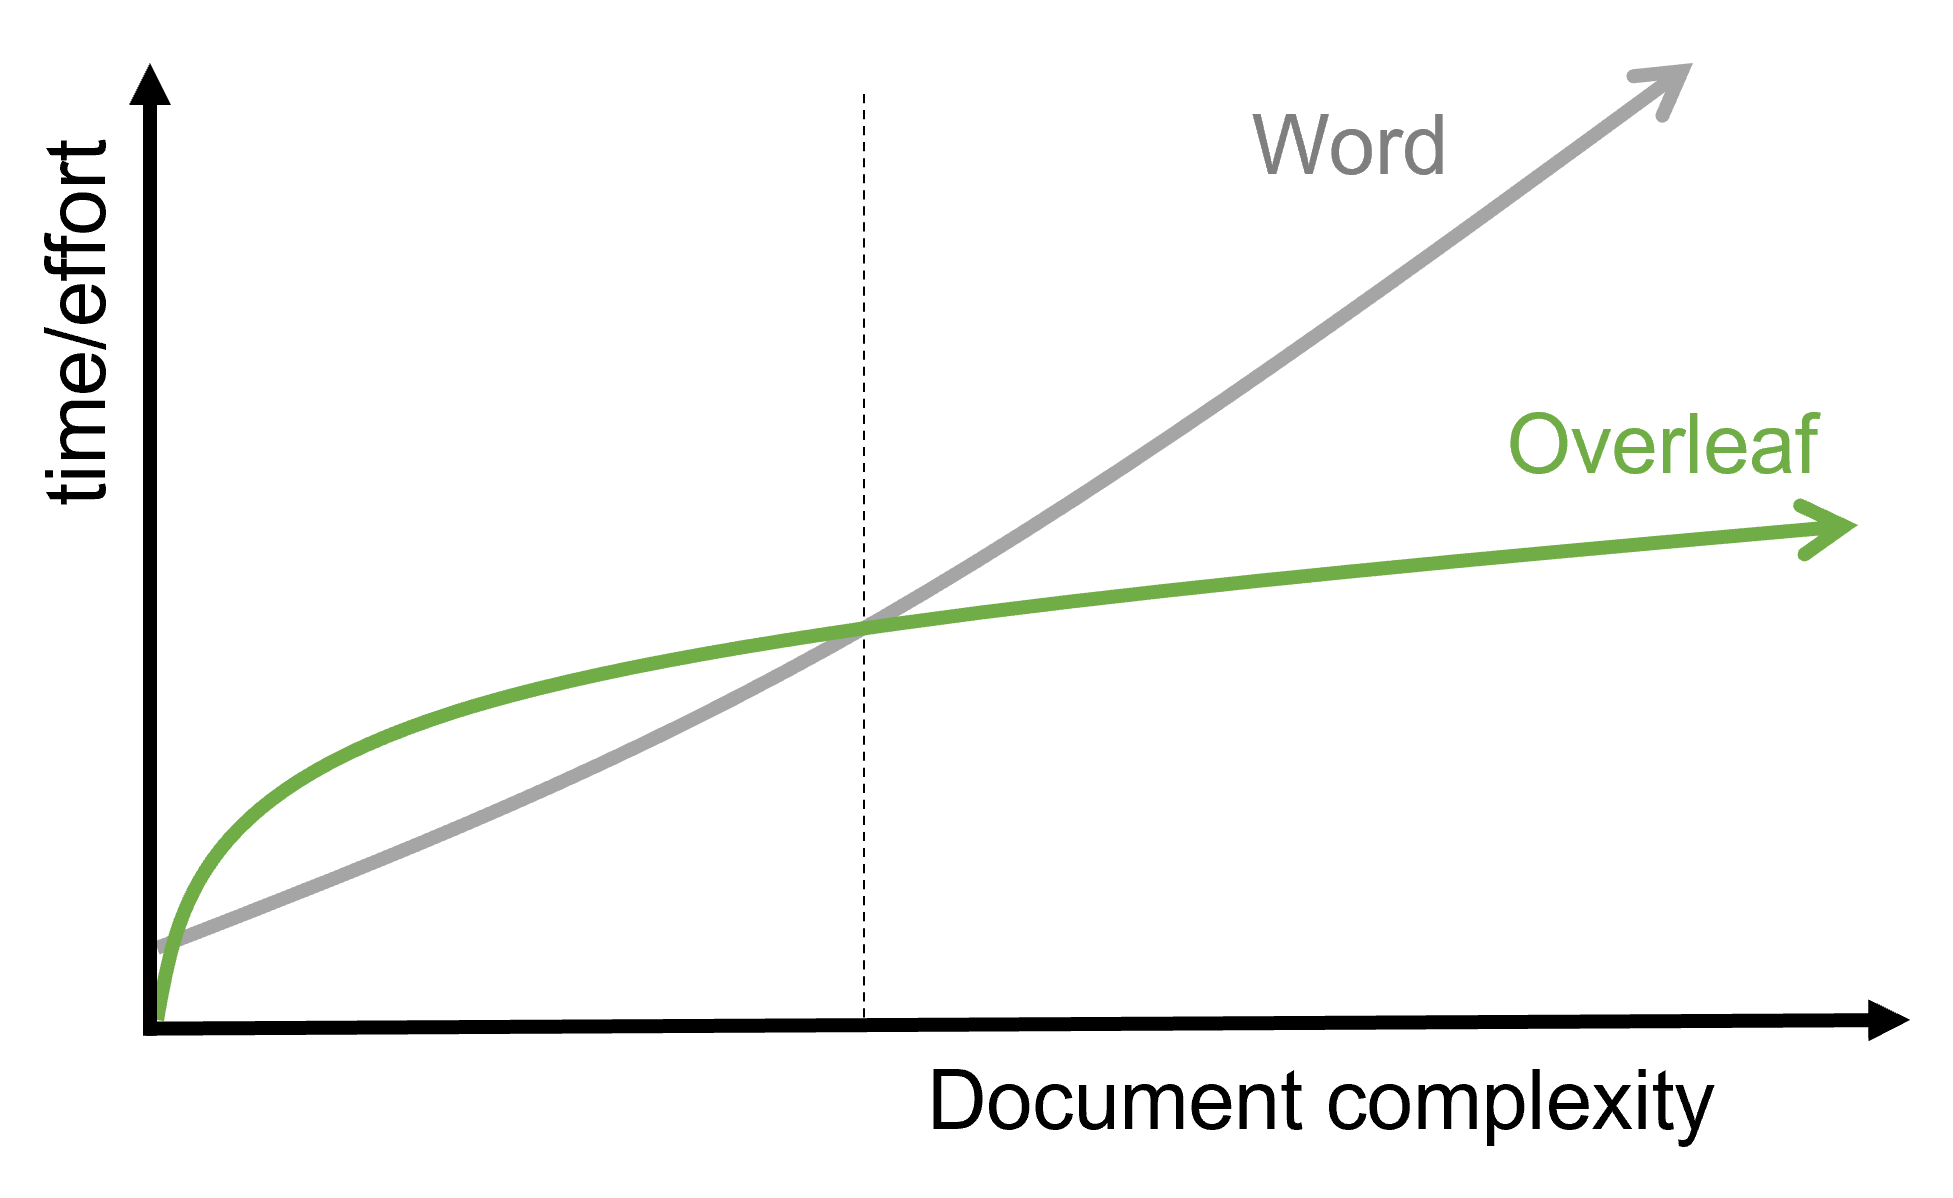
\includegraphics[width=0.8\textwidth,keepaspectratio]{images/v_word.png}
% source: https://tex.stackexchange.com/questions/1756/why-should-i-use-latex
\end{frame}


% new frame -------------------------------------------------
\section{Goal of Today}
\begin{frame}{Goal of Today}
 \begin{fullpageitemize}
    \item 1. Creating a project
    \item 2. Writing your work 
    \item 3. Collaborating with Others
 \end{fullpageitemize}
\end{frame}

% Creating a project %%%%%%%%%%%%%%%%%%%%%%%%%%%%%%%%%%%%%%%
\section{1. Creating a project}
\framepic[1]{images/seed}{
 \begin{textblock}{10}(0,-2.3)
    {\color{white}\hugetext{Creating a project}}
 \end{textblock}
}

% new frame -------------------------------------------------
\begin{frame}{1. Creating a project}

\green{\footnotesize{\url{https://www.overleaf.com/edu/utexas}}} \hfill \break


\includegraphics[width=\textwidth,keepaspectratio]{images/ut_overleaf.png}

\end{frame}


% new frame -------------------------------------------------
\subsection{Interface}
\begin{frame}{1. Creating a project - Interface}


\includegraphics[width=\textwidth,keepaspectratio]{images/ut_overleaf2.png}
\hfill \break

 \begin{fullpageitemize}
    \itemA \green{Templates} tab:\hfill \break

      \begin{fullpageitemize}
        \itemB Find the template you need (e.g., APA7 template)
        \itemB Use \green{Open as Template} to save it as your project
     \end{fullpageitemize}
     
    \itemA \green{Projects} tab: See your projects directly
 \end{fullpageitemize}

\end{frame}

% new frame -------------------------------------------------
\begin{frame}{1. Creating a project - Interface}
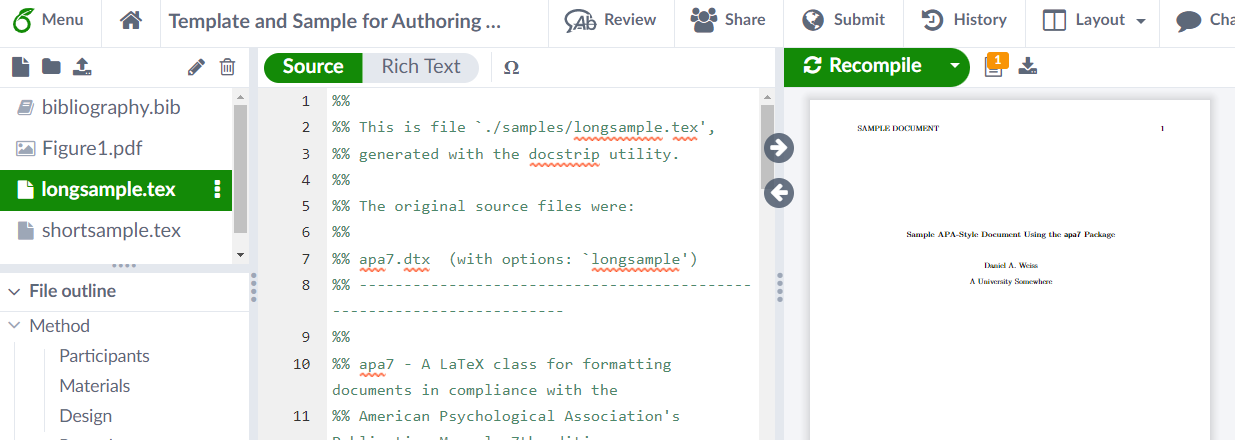
\includegraphics[width=\textwidth,keepaspectratio]{images/ut_overleaf3.png}

 \begin{fullpageitemize}
    \itemA \green{Menu} tab: Download the results, copy projects, etc.
    \itemA Left panel: Overview of files {\scriptsize(top)} and the document {\scriptsize(bottom)}
    \itemA Center panel: Writing area {\scriptsize(select \green{Source} or \green{Rich Text})}
    \itemA Right panel: The results {\scriptsize(click \green{Recompile}, Ctrl/Cmd + S, or Ctrl/Cmd + Enter)}
 \end{fullpageitemize}

\end{frame}

% new frame -------------------------------------------------
\subsection{Templates}
\begin{frame}{1. Creating a project - Templates} 

 \begin{fullpageitemize}
    \itemA QP
    \green{\scriptsize{\url{https://github.com/youngrilee/QM-QP-template}}}
    \itemA Dissertation \green{\scriptsize{\url{https://github.com/youngrilee/QM-dissertation-template}}}\hfill \break
    \begin{fullpageitemize}
    \itemB Click \green{Code} and then \green{Download ZIP}
    \end{fullpageitemize}
    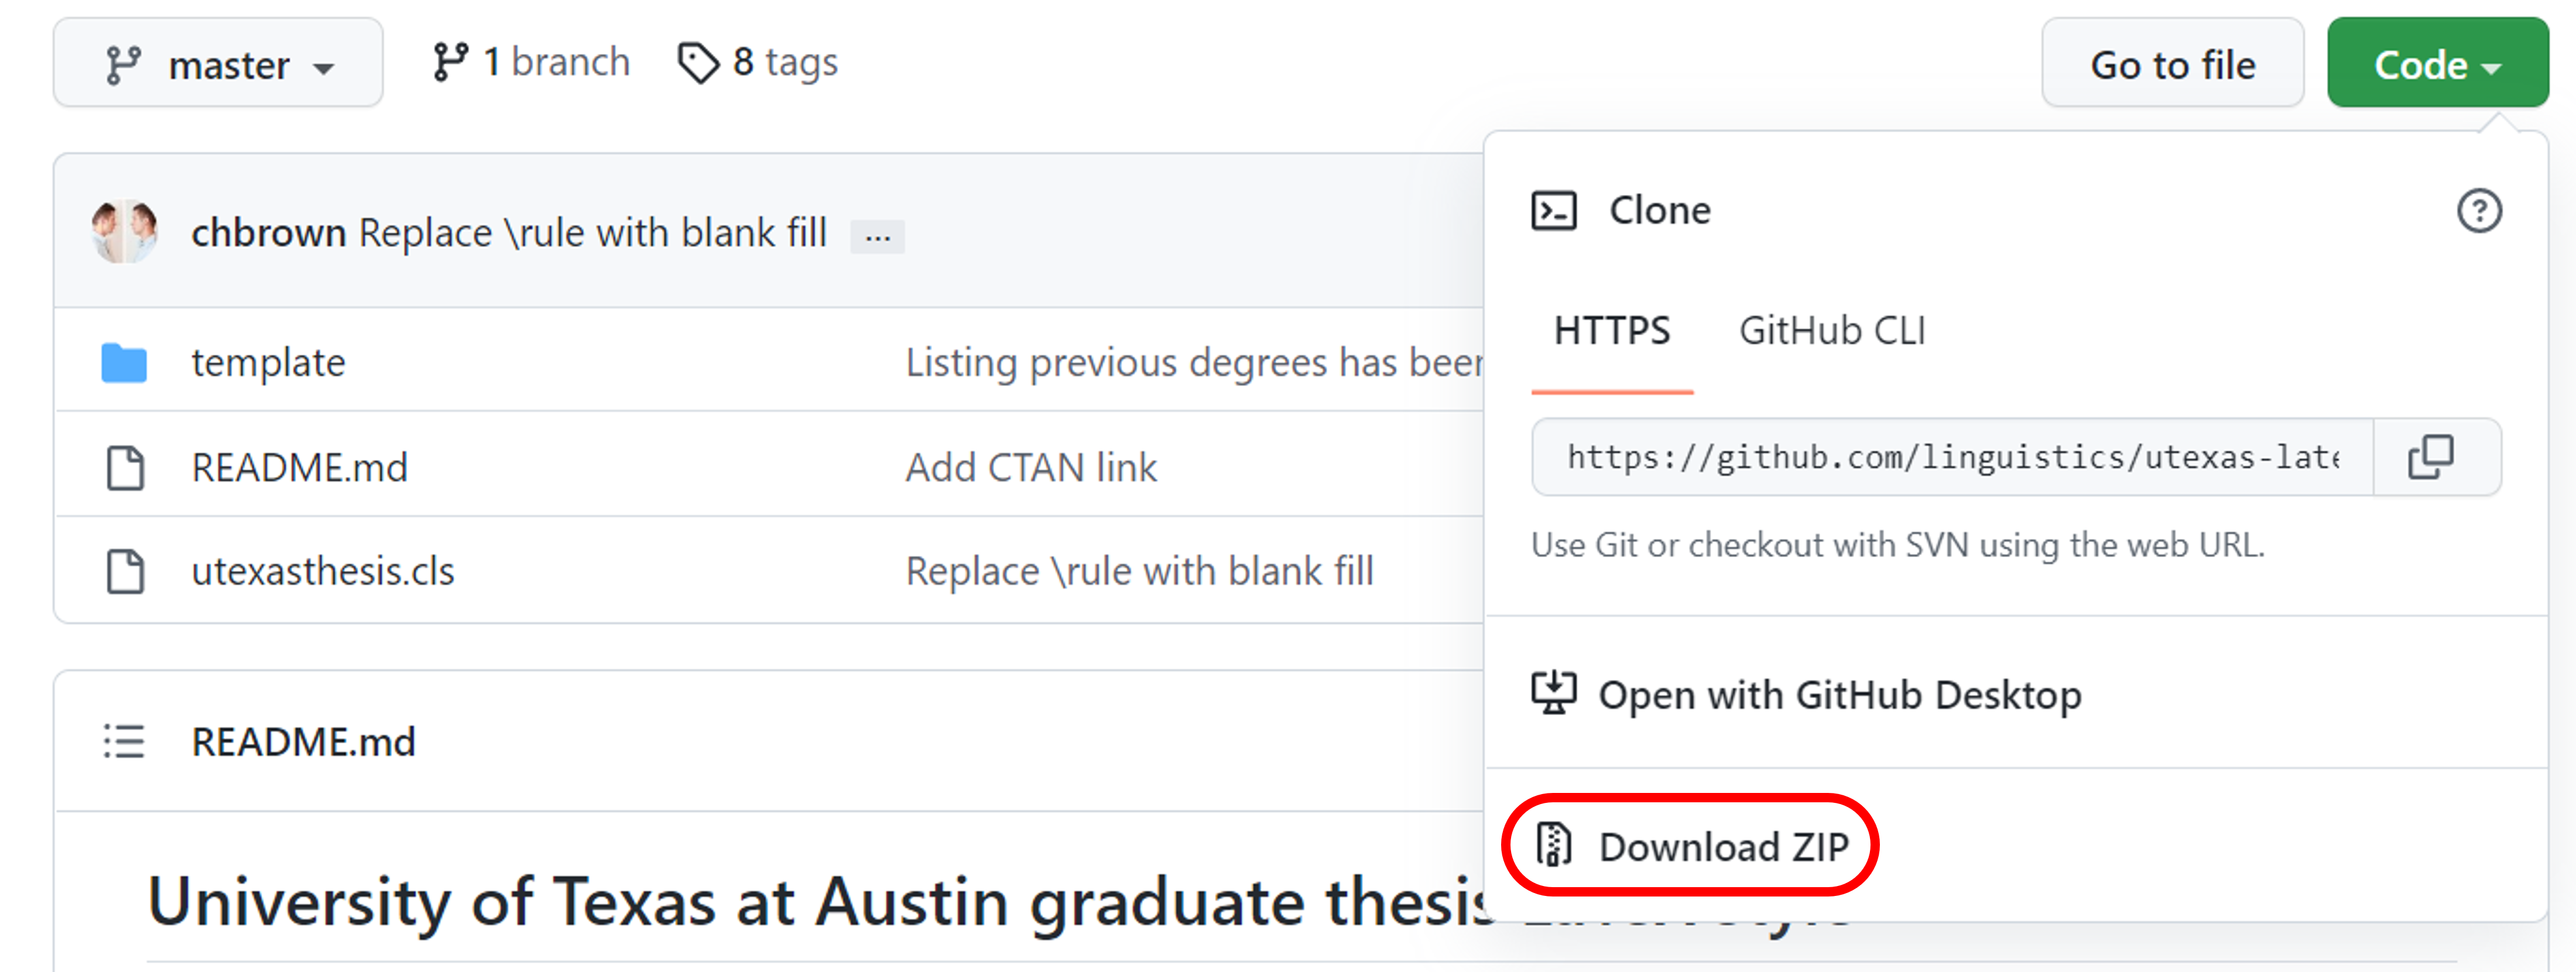
\includegraphics[width=0.9\textwidth,keepaspectratio]{images/git_download.png}
 \end{fullpageitemize}
 
\end{frame}

% new frame -------------------------------------------------
\begin{frame}{1. Creating a project - Templates} 

 \begin{fullpageitemize}
    \itemA  Click \green{Upload Project} and upload the .zip file \hfill \break 
    
    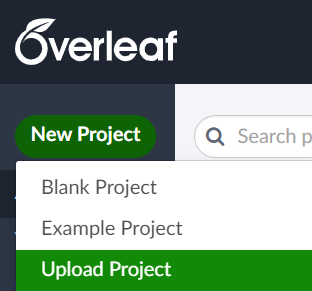
\includegraphics[width=0.4\textwidth,keepaspectratio]{images/upload_proj.png}
 \end{fullpageitemize}
 
\end{frame}

% Writing your work %%%%%%%%%%%%%%%%%%%%%%%%%%%%%%%%%%%%%%%%
\section{2. Writing your work}
\framepic[1]{images/create}{
 \begin{textblock}{10}(0,-2.3)
    {\color{white}\hugetext{Writing your work}}
 \end{textblock}
}

% new frame -------------------------------------------------
\begin{frame}{2. Writing your work}

 \begin{fullpageitemize}
    \itemA Figures
    \itemA Tables
    \itemA Equations
    \itemA Bibliographies
 \end{fullpageitemize}
\end{frame}

% new frame -------------------------------------------------
\begin{frame}{2. Writing your work - Basics}

 \begin{fullpageitemize}
    \itemA main.tex: Main document
    \itemA config.tex: Setup the style of the document
    \itemA The context of each section is included using \green{\textbackslash input}
    \itemA Basic commands to organize your content:\hfill \break
     \begin{fullpageitemize}
     {\footnotesize 
     \itemB \green{\textbackslash section}\{\textit{section title}\}
     \itemB \green{\textbackslash subsection}\{\textit{subsection title}\}
     \itemB \green{\textbackslash subsubsection}\{\textit{subsubsection title}\}
     \itemB \green{\textbackslash paragraph}\{\textit{paragraph title}\}
     \itemB \green{\textbackslash subparagraph}\{\textit{subparagraph title}\}
     }
     \end{fullpageitemize}
 \end{fullpageitemize}
\end{frame}

% new frame -------------------------------------------------
\begin{frame}{2. Writing your work - Basics}

 \begin{fullpageitemize}
    \itemA Basic commands for text formatting: \hfill \break
    \begin{fullpageitemize}
     \itemB {\footnotesize\texttt{\green{\textbackslash textbf}\{Bold\}}} \hspace{20mm} \textbf{Bold}\\
     \itemB {\footnotesize\texttt{\green{\textbackslash textit}\{Italics\}}} \hspace{15mm} \textit{Italics}\\
     \itemB {\footnotesize\texttt{\green{\textbackslash underline}\{Underline\}}} \hspace{8mm} \underline{Underline}
     \itemB {\footnotesize\texttt{\green{\textbackslash texttt}\{Monospace font\}}} \hspace{5mm} \texttt{Monospace font}
     \end{fullpageitemize}
 \end{fullpageitemize}
\end{frame}

% new frame -------------------------------------------------
\subsection{Figures}
\begin{frame}[fragile]{2. Writing your work - Figures}
\begin{fullpageitemize}
    \itemA Upload an image (.eps, .png, .jpeg)
    
    \itemA Simple example\\
    {\footnotesize
    \begin{verbatim}
    \includegraphics{figures/figure1.eps}
    \end{verbatim}
    }
    \itemA APA7 example
{\footnotesize
    \begin{verbatim}
    \begin{figure}[b!] 
        \centering
        \includegraphics[width=1.0\textwidth]{figures/figure1.eps}
        \caption{This is a figure.}
        \label{fig:fig1}
    \end{figure}
    \end{verbatim}
    }
    \begin{fullpageitemize}
    \itemB \green{[b!]} h (here), t (top), b (bottom) ! (float) 
    \itemB \green{[width=1.0\textbackslash textwidth]} Specify the size of the figure
    \end{fullpageitemize}
\end{fullpageitemize}

\end{frame}

% new frame -------------------------------------------------
\subsection{Tables}
\begin{frame}[fragile]{2. Writing your work - Tables}
\begin{fullpageitemize}
\itemA APA7 example
{\scriptsize
\begin{verbatim}
\begin{table}[b!]
\begin{center}\caption{This is a table.}\label{tab:table1}
\footnotesize
  \begin{tabular}{llcr}
     \textbf{Column} & \textbf{Column} & \textbf{Column} & \textbf{Column}\\      
     \hline
     \addlinespace[1ex]
     IV1 & 1 & Small  & 0 \\
         & 2 & Medium & 0 \\
         & 3 & Large  & 0  \\
     \addlinespace[1ex]
     \hline
  \end{tabular}

  \bigskip
  \footnotesize\textit{Note}. This table demonstrates..
\end{center}
\end{table}
\end{verbatim}
}
\end{fullpageitemize}
\end{frame}

% new frame -------------------------------------------------
\begin{frame}[fragile]{2. Writing your work - Tables}
\begin{fullpageitemize}
\itemA APA7 example \hfill \break
\begin{fullpageitemize}
    \itemB \green{\textbackslash label\{tab:table1\}}: Naming the table for future use in the document (e.g., Table \green{\textbackslash ref\{tab:table1\}} illustrates..) 
    \itemB \green{\&} Divide the columns in the table
    \itemB \green{\textbackslash \textbackslash} Finish a row in the table
    \itemB \green{\textbackslash begin\{tabular\}\{llcr\}}:\\ l (left-aligned) c (center) r (right-aligned)\\
    Should be the same number as the number of the columns in your table
    \end{fullpageitemize}
\end{fullpageitemize}
\end{frame}


% new frame -------------------------------------------------
\subsection{Equations}
\begin{frame}[fragile]{2. Writing your work - Equations}
\begin{fullpageitemize}
\itemA Basic Equations \hfill \break
{\scriptsize
\begin{verbatim}
\begin{equation}\label{hlm}
    Y_{ij} = \gamma_{00} + \gamma_{10}X_{ij} + \gamma_{01}W_j + b_{0j} + u_{ij}.
\end{equation}

Equation \ref{hlm} shows that..
\end{verbatim}
}
{\small
\begin{equation}\label{hlm}
    Y_{ij} = \gamma_{00} + \gamma_{10}X_{ij} + \gamma_{01}W_j + b_{0j} + u_{ij}.
\end{equation}
Equation \ref{hlm} shows that..}

\itemA Inline Equations \hfill \break
{\footnotesize
\begin{verbatim}
The intercept $\gamma_{00}$ indicates..
The intercept \(\gamma_{00}\) indicates..
\end{verbatim}}
{\small The intercept \(\gamma_{00}\) indicates..}
\end{fullpageitemize}
\end{frame}

% new frame -------------------------------------------------
\begin{frame}[fragile]{2. Writing your work - Equations}
\begin{fullpageitemize}
\itemA Other examples \hfill \break
{\scriptsize
\begin{verbatim}
\begin{equation}\label{ex1}
\begin{aligned}
    X & = \sqrt{\alpha^{2} + \beta^{2} + \frac{1}{2}} \\
    Y & = \sum_{n=1}^{N}{X_{n}} \\
    Z & =  \begin{pmatrix}
            1 & 2 & 3\\
            4 & 5 & 6 
            \end{pmatrix}
\end{aligned}
\end{equation}
\end{verbatim}
}
{\footnotesize
\begin{equation}\label{ex1}
\begin{aligned}
& X  = \sqrt{\alpha^{2} + \beta^{2} + \frac{1}{2}} \\
& Y  = \sum_{n=1}^{N}{X_{n}} \\
& Z  = 
\begin{pmatrix}
1 & 2 & 3\\
4 & 5 & 6 
\end{pmatrix}
\end{aligned}
\end{equation}
}
\end{fullpageitemize}
\end{frame}

% new frame -------------------------------------------------
\subsection{Bibliographies}
\begin{frame}{Bibliographies using \texttt{.bib} file}

 \begin{fullpageitemize}
    \itemA Create a \texttt{.bib} file and fill out \texttt{BibTeX} manually \hfill \break
    
    \begin{fullpageitemize}
    \itemB Click \green{New File}
    \itemB Create a file with \texttt{.bib} extension {\footnotesize e.g., \texttt{myReferences.bib}}
    \itemB Add references in \texttt{BibTex} format {\footnotesize(from Google Scholar, etc.)}
    \end{fullpageitemize}

\end{fullpageitemize}
\end{frame}

% new frame -------------------------------------------------
\begin{frame}{Bibliographies using \texttt{.bib} file}

 \begin{fullpageitemize}
        
    %\itemA \textcolor{gray}{Upload citations exported from Mendeley or Zotero}
    \itemA Link your account to Mendeley or Zotero \hfill \break
        \begin{fullpageitemize}
        \item [\textcolor{black}{\textopenbullet}]In \green{Account Settings}, connect to Mendeley or Zotero by logging-in \\ \hfill \break
        
\includegraphics[width=\textwidth,keepaspectratio]{images/ut_overleaf4.png}
        \end{fullpageitemize}
\end{fullpageitemize}

\end{frame}

% new frame -------------------------------------------------
\begin{frame}{Bibliographies using \texttt{.bib} file}

 \begin{fullpageitemize}
        
    \itemA Link to Mendeley or Zotero \hfill \break
        \begin{fullpageitemize}
        \item [\textcolor{black}{\textopenbullet}] In your project, click the \green{Upload} icon \\ \hfill \break
        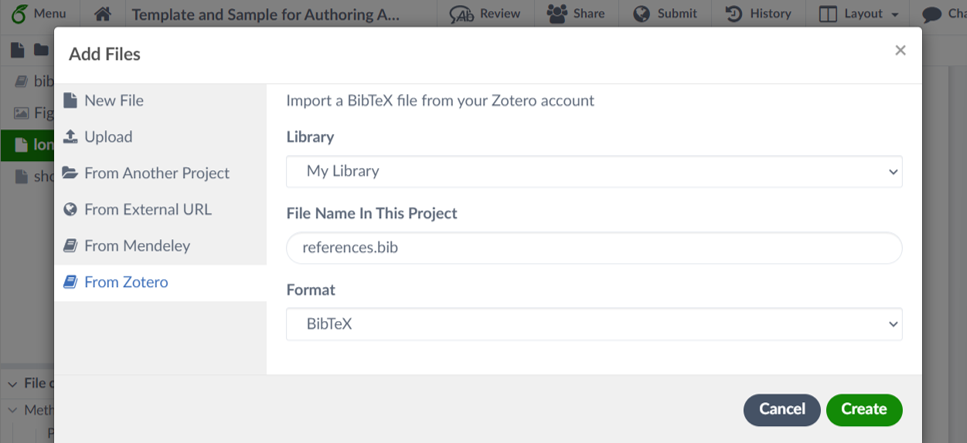
\includegraphics[width=\textwidth,keepaspectratio]{images/ut_overleaf5.png}
        \end{fullpageitemize}
\end{fullpageitemize}

\end{frame}

% new frame -------------------------------------------------
\begin{frame}{Bibliographies using \texttt{.bib} file}

 \begin{fullpageitemize}
        
    \itemA Once you have \texttt{.bib} file in your project, you are ready \hfill \break
        \begin{fullpageitemize}
        \item [\textcolor{black}{\textopenbullet}] Install \green{\texttt{biblatex}} package 
        {\scriptsize \texttt{\green{\textbackslash usepackage}[style=apa,sortcites=true,sorting=nyt,backend=biber]\{biblatex\}}}
        
        \item [\textcolor{black}{\textopenbullet}] Connect with the \texttt{.bib} file \\  {\footnotesize\texttt{\green{\textbackslash addbibresource}\{bibliography.bib\}}}
        \item [\textcolor{black}{\textopenbullet}] Cite \\ 
        {\footnotesize\texttt{\green{\textbackslash cite}\{cameron2015practitioner\}}} \hspace{10mm}
        {\latolightfont \cite{cameron2015practitioner}}\\
        {\footnotesize\texttt{\green{\textbackslash
        textcite}\{cameron2015practitioner\}}} \hspace{4mm}
        {\latolightfont \textcite{cameron2015practitioner}}\\
        {\footnotesize \texttt{\green{\textbackslash
        parencite}\{cameron2015practitioner\}}} \hspace{2mm}
        {\latolightfont \parencite{cameron2015practitioner}}\\
        
        \item [\textcolor{black}{\textopenbullet}] Add reference list\\
        {\footnotesize \texttt{\green{\textbackslash printbibliography}}}
        
        
        \end{fullpageitemize}
\end{fullpageitemize}

\end{frame}

% Collaborate with Others %%%%%%%%%%%%%%%%%%%%%%%%%%%%%%%%%%%%%%%%
\section{3. Collaborate with Others}
\framepic[1]{images/team}{
 \begin{textblock}{10}(2.5,2.5)
    {\color{white}\hugetext{\textbf{Collaborating with Others}}}
 \end{textblock}
}

% new frame -------------------------------------------------
\begin{frame}{3. Collaborating with Others}
 \begin{fullpageitemize}
    \itemA Track Changes
    \itemA Insert comments
    \itemA Exporting your work
 \end{fullpageitemize}
\end{frame}

% new frame -------------------------------------------------
\subsection{Track Changes}
\begin{frame}{3. Collaborating - Track Changes}

\includegraphics[width=\textwidth,keepaspectratio]{images/share.png}
    \hfill \break
 \begin{fullpageitemize}
    \itemA \green{Share}: Share your project (select \green{Can Edit} option) 
    \itemA Select \green{Review}
    \itemA Turn the \green{track changes} on/off using the toggle buttons
 \end{fullpageitemize}
\end{frame}

% new frame -------------------------------------------------
\subsection{Insert Comments}
\begin{frame}{3. Collaborating - Insert Comments}

\includegraphics[width=\textwidth,keepaspectratio]{images/comment.png}
    \hfill \break
 \begin{fullpageitemize}
    \itemA Anyone who reads the article can use the comment feature
    \itemA Drag the sentence you want and select  \green{Add comment}
    \itemA Collaborators can reply to others' comments
    \itemA Comments can be edited, resolved, re-opened, or permanently deleted
 \end{fullpageitemize}
\end{frame}

% new frame -------------------------------------------------
\subsection{Exporting}
\begin{frame}{3. Collaborating - Exporting your work}

 \begin{fullpageitemize}
    \itemA \green{Menu}
    \hfill \break
    \begin{fullpageitemize}
    \itemBDownload as \texttt{.zip} file
    \itemBDownload as \texttt{.pdf} file
    \end{fullpageitemize}
    
\includegraphics[width=0.3\textwidth,keepaspectratio]{images/download.png}
    \itemA FYI, you can submit to \textit{arXiv} using the \green{Submit} feature \hfill \break
    
\includegraphics[width=0.8\textwidth,keepaspectratio]{images/submit.png}
 \end{fullpageitemize}
\end{frame}


% new frame -------------------------------------------------
\section{Wrap-up}
\begin{frame}{Wrap-up}
1. Creating a project
     \begin{itemize}
         \item [\textcolor{black}{\textbullet}] Interface
         \item [\textcolor{black}{\textbullet}] QP and dissertation templates
     \end{itemize} \hfill \break
2. Writing your work 
     \begin{itemize}
         \itemA Figures, tables, and equations 
         \itemA Adding references
     \end{itemize} \hfill \break
3. Collaborating with Others 
     \begin{itemize}
         \itemA Track changes and adding comments
         \itemA Exporting your work
     \end{itemize}
\end{frame}

% new frame -------------------------------------------------
\section{Resources}
\begin{frame}{Resources}
 \begin{fullpageitemize}
 \small
 \itemA\green{\url{https://www.overleaf.com/learn}}
 \itemA\green{\url{https://www.overleaf.com/events/webinars}}
 \itemA \green{\url{https://www.overleaf.com/learn/latex/Free_online_introduction_to_LaTeX_(part_1)}}
 \itemA Google and StackExchange are your friends!
 \end{fullpageitemize}
\end{frame}

% Thank you %%%%%%%%%%%%%%%%%%%%%%%%%%%%%%%%%%%%%%%%
\framepic[1]{images/coffee}{
 \begin{textblock}{10}(0,-2.3)
    {\color{white}\hugetext{Thank you!}}
 \end{textblock}
  \begin{textblock}{10}(4,3.9)
    {\color{white}\hugetext{Any Questions?}}
 \end{textblock}
}

%\begin{frame}{Presento}
% \begin{fullpageitemize}
%  \item \begin{center}\largetext{The design is \underline{clean}}\end{center}
%  \item \begin{center}\largetext{The rules are \underline{simple}}\end{center}
%  \item \begin{center}\largetext{The code is \underline{extensible}}\end{center}
% \end{fullpageitemize}
%\end{frame}

%\begin{frame}{Open Source Fonts}
% \begin{fullpageitemize}
%  \item {\montserratfont This is Montserrat}
%  \item {\notosansfont This is Noto Sans}
%  \item {\latolightfont This is Lato (light)}
%  \item {\inconsolatafont This is inconsolata}
%  \item \textsc{This is Alegreya Sans small caps}
% \end{fullpageitemize}
%\end{frame}

%\begin{frame}{Color Palette}
% \begin{center}
%  \crule[colordgray] \crule[colorhgray] \crule[colorblue] \crule[colorgreen] \crule[colororange]
% \end{center}
%\end{frame}

%\framecard[colorgreen]{{\color{white}\hugetext{Thank You}}}

\end{document}